We computed the posterior of $(D,r)$ for this equation. The interval is $[0,60]$ with Neumann ends, the initial condition $u(0,x)=\tfrac12\operatorname{erfc}\big(\sqrt2\,(x-5)\big)$ is a step smoothed by a Gaussian, known and fixed, and the truth is $D=r=1$, so that the speed $c^*=2\sqrt{rD}$ is $2$ and the width $w=\sqrt{D/r}$ is $1$. The data are $u$ at $72$ sensors $x=0.5,1,\dots,36$ and $48$ times $t=0.25,0.5,\dots,12$ with independent Gaussian errors of standard deviation $\delta=0.05$, observed in the nested windows $[0,T]$ with $T=0.5$, $3$ and $12$, which hold $144$, $864$ and $3456$ values. The prior of $(\log D,\log r)$ is Gaussian with medians $(0.5,0.7)$ and standard deviation $1$ in each coordinate, so it is centered away from the truth. The forward map is a method of lines with a cosine transform in $x$, which makes diffusion exact, combined with the closed form flow of the logistic term by Strang splitting, with grid spacing $0.1$ and time step $0.0125$. At the data points it differs by at most $6\times10^{-6}$ both from the same scheme at half the spacing and step and from an independent finite difference solver; the data are generated with the finite difference solver, so the posterior is not computed with the discretization that made the data. The log posterior changes by at most $0.003$ at sample nodes of the region that carries $99.9$ percent of its mass when either replaces the solver. The speed of the half height point of the front is $0.927\,c^*$ at $rt=12$ and $0.960\,c^*$ at $rt=20$, against $0.9375\,c^*$ and $0.9625\,c^*$ from the logarithmic delay $c^*\big(1-3/(4rt)\big)$ of pulled fronts~\cite{bramson1983,ebert2000}.

We evaluate the posterior of $(\log D,\log r)$ exactly on a grid of at least $61\times61$ nodes along its principal axes, once for each window, with no Markov chain; dropping every second node changes the means and standard deviations by less than $2\times10^{-4}$ posterior standard deviations. Figure~\ref{fig:fk_posterior} and Table~\ref{tab:fk_posterior} give the result. Both parameters are identified, increasingly well as the window grows, and the speed is identified better than the width. The posterior at $T=12$ is a ridge close to the curve $Dr=\mathrm{const}$, along which the speed is fixed and the width varies, and tilted by $12$ degrees from it toward the $\log D$ axis. The tilt shrinks slowly with the window ($12$, $10$ and $8.5$ degrees at $T=12$, $18$ and $24$ in the linearization at the truth). The ridge follows the parameters that leave the front trajectory unchanged to first order: the Fisher information of the position of the half height point of the front, as a function of time, has its long axis at $147.8$ degrees, against $147.4$ for all the data, and the sign of the tilt is that of the logarithmic delay, since a wider front lags farther behind the line $x=c^*t+\mathrm{const}$ and is offset by a slightly larger speed. Before a front has formed the picture is different. At $T=0.5$ the half height point moves at $0.30\,c^*$ over the second half of the window, against $0.62\,c^*$ and $0.89\,c^*$ for the other two windows, and the reaction term changes the solution by only $0.3$ noise standard deviations rms over the data. The posterior is a broad region, skewed toward small $r$, whose long axis lies within $10$ degrees of the $\log r$ axis, the direction of constant $D$: $D$ is determined to $17$ percent and $r$ to $30$ percent, but there is no ridge. As the window grows the contours therefore pass from a broad region to a ridge. In the linearization at two other truths, $(0.5,1.5)$ and $(2,0.5)$, the correlation goes from $-0.28$ and $-0.10$ at $T=0.5$ to $-0.98$ and $-0.89$ at $T=12$.

A Gaussian approximation at the posterior mode, which a variational method with an adjoint model can deliver, has standard deviations within $1$ percent of the exact ones for $T=3$ and $12$, but at $T=0.5$ gives $0.245$ for $\log r$ instead of $0.298$ and misses the skew (dotted curve in the figure). To check calibration we repeated the experiment with $1000$ other noise draws: the exact $90$ percent regions contain the truth in $92.2$, $88.8$ and $89.0$ percent of the draws (standard error $0.9$ percent), and the $50$ percent regions in $55.0$, $50.6$ and $50.2$ percent; for the draw in the figure the truth lies just outside the $90$ percent region at $T=3$, in the $92$ percent region, which is within this variation. We also compared a small conditional generator, of the kind in Proposition~\ref{prop:bvm_generators}, with the exact posterior. It is a triangular map of two quantile networks, one for $\log D$ given the summary and one for $\log r$ given the summary and $\log D$, trained by the check loss on simulated pairs $(\theta,y)$; the two dimensional summary is $s=J^\top\big(y-\mathcal{G}(\hat\theta)\big)/\delta^2$ with $J$ the Jacobian of $\mathcal{G}$ at the posterior mode $\hat\theta$, the gradient of the data misfit, which costs one adjoint solve in a partial differential equation problem. Trained on $20000$ pairs whose parameters are uniform on a region of $4.5$ standard deviations of the Gaussian approximation around $\hat\theta$ (weighted by the prior density), with three training seeds, its means differ from the exact ones by at most $0.04$ exact standard deviations at both $T=12$ and $T=3$, and its standard deviations by at most $2$ percent at $T=12$ and $8$ percent at $T=3$, although the spread across the ridge at $T=12$ is $5$ to $7$ percent too large (bottom right of the figure); with $1000$ or $4000$ pairs the standard deviations at $T=12$ are $2$ to $9$ percent too small. Trained on draws from the prior instead, it is $4$ exact standard deviations off at $T=12$, with spreads $11$ to $12$ times too large, while at $T=3$ it is within $0.2$ standard deviations, with spreads $10$ to $20$ percent too large. The proposal around $\hat\theta$ uses the data, so the generator is local to one data set, and the experiment does not show that a generator trained on the prior reproduces a narrow posterior. The exact posteriors are for one truth, one design and a known initial condition, so the experiment says nothing about recovering the initial condition.

\begin{figure}[t]
\centering
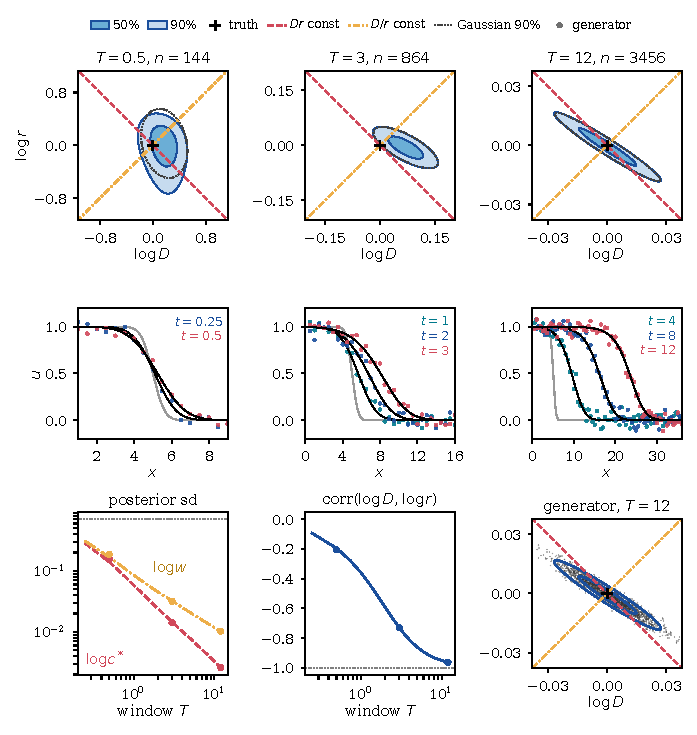
\includegraphics[width=\textwidth]{fk_posterior}
\caption{Exact posterior of $(\log D,\log r)$ for the Fisher Kolmogorov equation with $D=r=1$ and three nested observation windows $[0,T]$ with $n$ values; the axis scales differ. Top: $50$ and $90$ percent highest posterior density regions, the truth, the curves $Dr=\mathrm{const}$ (front speed) and $D/r=\mathrm{const}$ (front width) through it, and the $90$ percent region of the Gaussian approximation at the posterior mode (dotted). Middle: data (dots), solution at the posterior mean (black) and initial condition (gray). Bottom: posterior standard deviations of $\log c^*$ and $\log w$, with $c^*=2\sqrt{rD}$ and $w=\sqrt{D/r}$, and correlation of $(\log D,\log r)$ from the linearization at the truth as the window grows, with the exact values at the three windows (dots) and the prior standard deviation of $\log c^*$ and $\log w$ (dotted line); and $2000$ draws of a generator trained on $20000$ simulations, with the exact contours, for $T=12$.}
\label{fig:fk_posterior}
\end{figure}

\begin{table}[t]\centering\small
\caption{Exact posterior of $(\log D,\log r)$ by observation window: standard deviations $\sigma_D$ and $\sigma_r$ of $\log D$ and $\log r$, their correlation $\rho$, the ratio of the lengths of the principal axes of the contours, the angle of the long axis from the $\log D$ axis in degrees ($135$ is the curve $Dr=\mathrm{const}$ and $45$ the curve $D/r=\mathrm{const}$), and the standard deviations $\sigma_c$ and $\sigma_w$ of $\log c^*$ and $\log w$. The prior standard deviation of $\log D$ and $\log r$ is $1$.}\label{tab:fk_posterior}
\begin{tabular}{rrrrrrrr}
\toprule
$T$ & $\sigma_D$ & $\sigma_r$ & $\rho$ & ratio & angle & $\sigma_c$ & $\sigma_w$\\
\midrule
$0.5$ & $0.170$ & $0.298$ & $-0.21$ & $1.8$ & $100$ & $0.156$ & $0.186$\\
$3$ & $0.0412$ & $0.0263$ & $-0.73$ & $2.9$ & $151$ & $0.0142$ & $0.0315$\\
$12$ & $0.0125$ & $0.0081$ & $-0.96$ & $8.1$ & $147$ & $0.0026$ & $0.0103$\\
\bottomrule
\end{tabular}
\end{table}
